\documentclass[12pt]{article}

% Layout.
\usepackage[top=1.2in, bottom=0.75in, left=1in, right=1in, headheight=1.0in, headsep=0pt]{geometry}

% Fonts.
\usepackage{mathptmx}
\usepackage[scaled=0.86]{helvet}
\renewcommand{\emph}[1]{\textsf{\textbf{#1}}}

% TiKZ.
\usepackage{tikz, pgfplots}
\usetikzlibrary{calc}
\pgfplotsset{my style/.append style={axis x line=middle, axis y line=middle, xlabel={$x$}, ylabel={$y$}}}
\pgfplotsset{compat=1.16}

% Misc packages.
\usepackage{amsmath,amssymb,latexsym,bm,array,multicol,enumitem}
\usepackage{graphicx}
\usepackage{xcolor}
\usepackage[most]{tcolorbox}
\usepgfplotslibrary{fillbetween}
\definecolor{solbg}{RGB}{225,240,252}
\definecolor{solframe}{RGB}{70,130,180}
\newtcolorbox{solution}[1][]{%
  breakable, enhanced,
  colback=solbg, colframe=solframe, boxrule=0.7pt, arc=3pt,
  left=6pt, right=6pt, top=5pt, bottom=5pt,
  before skip=6pt, after skip=6pt,
  fonttitle=\sffamily\bfseries\small, coltitle=white, title={Solution},
  #1}

% Commands to set various header/footer components.
\makeatletter
\def\doctitle#1{\gdef\@doctitle{#1}}
\doctitle{Use {\tt\textbackslash doctitle\{MY LABEL\}}.}
\def\docdate#1{\gdef\@docdate{#1}}
\docdate{Use {\tt\textbackslash docdate\{MY DATE\}}.}
\def\doccourse#1{\gdef\@doccourse{#1}}
\let\@doccourse\@empty
\def\docscoring#1{\gdef\@docscoring{#1}}
\let\@docscoring\@empty
\def\docversion#1{\gdef\@docversion{#1}}
\let\@docversion\@empty
\makeatother

% Headers and footers layout.
\makeatletter
\usepackage{fancyhdr}
\pagestyle{fancy}
\fancyhf{} % Clears all headers/footers.
\lhead{\emph{\@doctitle\hfill\@docdate} \medskip
\ifnum \value{page} > 1\relax\else\\
\emph{Name: \rule{3.5in}{1pt}\hfill \@docscoring}
\fi}

\rfoot{\emph{\@docversion}}
\lfoot{\emph{\@doccourse}}
\cfoot{\emph{\thepage}}
\renewcommand{\headrulewidth}{0pt}%
\makeatother

% Paragraph spacing
\parindent 0pt
\parskip 6pt plus 1pt

% A problem is a section-like command. Use \problem{5} for a problem worth 5 points.
\newcounter{probcount}
\newcounter{subprobcount}
\setcounter{probcount}{0}

\newcommand{\problem}[1]{%
\par
\addvspace{4pt}%
\setcounter{subprobcount}{0}%
\stepcounter{probcount}%
\makebox[0pt][r]{\emph{\arabic{probcount}.}\hskip1ex}\emph{[#1 points]}\hskip1ex}

\newcommand{\thesubproblem}{\emph{\alph{subprobcount}.}}

% Subproblems are an enumerate-like environment with a consistent
% numbering scheme.  Use \begin{subproblems}\item...\item...\end{subproblems}
\newenvironment{subproblems}{%
\begin{enumerate}[itemindent=8pt,leftmargin=0pt]%
\setcounter{enumi}{\value{subprobcount}}%
\renewcommand{\labelenumi}{\emph{\textsl{\alph{enumi})}} \,}%
}%
{%
\setcounter{subprobcount}{\value{enumi}}%
\end{enumerate}%
}

% Blanks for answers in normal and math mode.
\newcommand{\blank}[1]{\rule{#1}{0.75pt}}
\newcommand{\mblank}[1]{\underline{\hspace{#1}}}
\def\emptybox(#1,#2){\framebox{\parbox[c][#2]{#1}{\rule{0pt}{0pt}}}}

% Misc.
\renewcommand{\d}{\displaystyle}
\newcommand{\ds}{\displaystyle}
\newcommand{\threeopts}{{\small \hspace{-6mm} $\begin{matrix} \text{\textsc{converges}} \\ \text{\textsc{absolutely}} \end{matrix}$ \qquad\qquad $\begin{matrix} \text{\textsc{converges}} \\ \text{\textsc{conditionally}} \end{matrix}$ \qquad\qquad \textsc{diverges}} \bigskip}


\newcommand{\ba}{\mathbf{a}}
\newcommand{\bb}{\mathbf{b}}
\newcommand{\bc}{\mathbf{c}}
\newcommand{\bi}{\mathbf{i}}
\newcommand{\bj}{\mathbf{j}}
\newcommand{\bk}{\mathbf{k}}
\newcommand{\bn}{\mathbf{n}}
\newcommand{\br}{\mathbf{r}}
\newcommand{\bu}{\mathbf{u}}
\newcommand{\bv}{\mathbf{v}}
\newcommand{\bw}{\mathbf{w}}

\newcommand{\bT}{\mathbf{T}}

\newcommand{\ip}[2]{\mathrm{\left<#1,#2\right>}}
\newcommand{\vv}[2]{\mathrm{\left<#1,#2\right>}}
\newcommand{\vvv}[3]{\mathrm{\left<#1,#2,#3\right>}}


\doctitle{Math 252: Midterm 1 Solutions}
\docdate{1 October, 2026}
\doccourse{}
\docversion{Solutions}
\docscoring{\fbox{{\LARGE \strut}\hspace{0.8in} / 100}}

\begin{document}
90 minutes maximum.  No aids (book, calculator, etc.) are permitted.
Show all work and use proper notation for full credit.  Answers should
be in reasonably-simplified form.  100 points possible.

\begin{enumerate}

\item Consider the region in the first quadrant bounded by the curves
  $\ds y = \sqrt{1-x^2}$, $x=0$, and $y=0$.
  \begin{enumerate}
  \item (4 points) Sketch the graph of the region. Be sure to clearly label
    any important points.
    \begin{solution}
      \begin{center}
      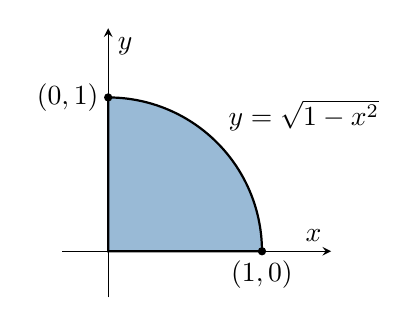
\begin{tikzpicture}
        \begin{axis}[my style, axis on top, width=5cm, height=5cm,
            xmin=-0.3, xmax=1.45, ymin=-0.3, ymax=1.45,
            xtick=\empty, ytick=\empty, axis equal image, clip=false]
          \addplot[domain=0:90, samples=60, fill=solframe, fill opacity=0.55,
            draw=black, thick] ({cos(x)}, {sin(x)}) -- (axis cs:0,0) -- cycle;
          \fill (axis cs:1,0) circle (1.5pt);
          \fill (axis cs:0,1) circle (1.5pt);
          \node[below] at (axis cs:1,0) {$(1,0)$};
          \node[left] at (axis cs:0,1) {$(0,1)$};
          \node[above right] at (axis cs:0.72,0.72) {$y=\sqrt{1-x^2}$};
        \end{axis}
      \end{tikzpicture}
      \end{center}
    \end{solution}
    \vfill

  \item (6 points) Write an integral that computes the volume of the solid
    obtained by rotating the region about the $x$-axis using the
    disk/washer method. {\bf Do not compute the integral}.
    \begin{solution}
      Disks of radius $\sqrt{1-x^2}$ for $0 \le x \le 1$:
      \[
        \boxed{V = \int_0^1 \pi\big(\sqrt{1-x^2}\big)^2\,dx}
      \]
    \end{solution}
    \vfill

  \item (6 points) Write an integral that computes the volume of the solid
    obtained by rotating the region about the $x$-axis using the method of
    cylindrical shells. {\bf Do not compute the integral}.
    \begin{solution}
      Cylindrical shells at height $y$ have radius $y$ and height $x = \sqrt{1-y^2}$,
      for $0 \le y \le 1$:
      \[
        \boxed{V = \int_0^1 2\pi y\sqrt{1-y^2}\,dy}
      \]
    \end{solution}
    \vfill

    \newpage

  \item (6 points) Compute one of the integrals from the previous two parts of
    this problem. You may choose which one to compute, but you must
    clearly indicate which one you have chosen.
    \begin{solution}
      Disk/washer integral from part (b):
      \[
        V = \pi\int_0^1 (1-x^2)\,dx = \pi\left[x - \frac{x^3}{3}\right]_0^1
        = \boxed{\frac{2\pi}{3}}.
      \]

      \medskip\emph{Alternative (cylindrical shells, part (c)).} With $u = 1-y^2$,
      $du = -2y\,dy$:
      \[
        \int_0^1 2\pi y\sqrt{1-y^2}\,dy = -\pi\int_1^0 u^{1/2}\,du
        = \pi\left[\frac23 u^{3/2}\right]_0^1 = \frac{2\pi}{3}.\quad\checkmark
      \]
    \end{solution}
    \vfill
    \vfill

  \item (4 points) How could you have calculated the volume from the previous
    parts {\bf without using calculus}?
    \begin{solution}
      The solid is a hemisphere of radius 1, so its volume is half that of a sphere:
      \[
        V = \frac12\cdot\frac43\pi(1)^3 = \boxed{\frac{2\pi}{3}}.
      \]
    \end{solution}
    \vfill

  \end{enumerate}


\item (6 points) Set up, but {\bf do not evaluate} an integral that computes the
  arc length of the curve $\ds y=e^{3x}$ between the points $\ds (0,1)$
  and $\left( \frac{1}{3}, e \right)$.
  \begin{solution}
    $y' = 3e^{3x}$, so
    \[
      \boxed{L = \int_0^{1/3} \sqrt{1 + 9e^{6x}}\,dx}
    \]
  \end{solution}
  \vfill
  \newpage

\item (10 points) A spring has a natural length of 2 meters. It requires 60 joules
  of work to stretch the spring to a length of 3 meters. How much would
  the spring stretch if you applied 15 joules of work? You
  may take Hooke's law ($F=kx$) as given, but must justify the rest of
  your answer with calculus.
  \begin{solution}
    Let $x$ be the stretch beyond the natural length, so 3 m is $x = 1$, and let $d$ be
    the stretch produced by 15 J:
    \[
      60 = \int_0^1 kx\,dx = \frac{k}{2} \;\Rightarrow\; k = 120;
      \qquad
      15 = \int_0^d 120x\,dx = 60d^2 \;\Rightarrow\; d^2 = \frac14.
    \]
    The spring stretches $\boxed{\tfrac12\ \text{meter}}$.
  \end{solution}
  \vfill

\item Consider the region bounded by $y = x^2$ and $y = \sqrt{x}$.
  \begin{enumerate}
  \item (4 points) Sketch the region. Be sure to clearly label any important points.
    \begin{solution}
      Intersections: $x^2 = \sqrt{x} \;\Rightarrow\; x^4 = x \;\Rightarrow\; x(x^3-1) = 0
      \;\Rightarrow\; x = 0,\ 1$, giving $(0,0)$ and $(1,1)$.

      \begin{center}
      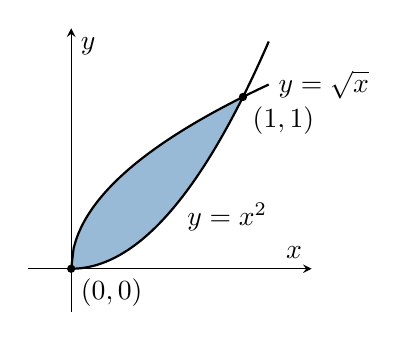
\begin{tikzpicture}
        \begin{axis}[my style, axis on top, width=5cm, height=5cm,
            xmin=-0.25, xmax=1.4, ymin=-0.25, ymax=1.4, scale only axis, width=3.6cm, height=3.6cm,
            xtick=\empty, ytick=\empty, axis equal image, clip=false]
          \addplot[name path=top, domain=0:1.15, samples=80, thick] {sqrt(x)};
          \addplot[name path=bot, domain=0:1.15, samples=80, thick] {x^2};
          \addplot[fill=solframe, fill opacity=0.55, draw=none]
            fill between[of=top and bot, soft clip={domain=0:1}];
          \fill (axis cs:1,1) circle (1.5pt);
          \fill (axis cs:0,0) circle (1.5pt);
          \node[below right] at (axis cs:1,1) {$(1,1)$};
          \node[below right] at (axis cs:0,0) {$(0,0)$};
          \node[right] at (axis cs:1.15,1.07) {$y=\sqrt{x}$};
          \node[right] at (axis cs:0.62,0.3) {$y=x^2$};
        \end{axis}
      \end{tikzpicture}
      \end{center}
    \end{solution}
    \vfill

  \item (8 points) Set up expressions for the
    centroid (center of mass) of the region. {\bf Do not evaluate} any
    integrals in your expressions.
    \begin{solution}
      On $0 \le x \le 1$ the top curve is $y = \sqrt{x}$ and the bottom is $y = x^2$.
      \[
        \boxed{\bar{x} = \frac{\ds\int_0^1 x\big(\sqrt{x} - x^2\big)\,dx}{\ds\int_0^1 \big(\sqrt{x} - x^2\big)\,dx}}
        \qquad
        \boxed{\bar{y} = \frac{\ds\int_0^1 \tfrac12\Big(\big(\sqrt{x}\big)^2 - \big(x^2\big)^2\Big)\,dx}{\ds\int_0^1 \big(\sqrt{x} - x^2\big)\,dx}}
      \]
    \end{solution}
    \vfill

  \end{enumerate}


    \newpage

\item Evaluate the following integrals and antiderivatives.
  \begin{enumerate}
  \item (8 points) $\ds \int_0^{\pi} x \sin(x) \, dx$
    \begin{solution}
      Integration by parts with $u = x$, $dv = \sin x\,dx$, $du = dx$, $v = -\cos x$:
      \begin{align*}
        \int_0^{\pi} x\sin x\,dx &= \Big[-x\cos x\Big]_0^{\pi} + \int_0^{\pi}\cos x\,dx \\[4pt]
          &= (-\pi\cos\pi - 0) + \Big[\sin x\Big]_0^{\pi} = \pi + 0 = \boxed{\pi}.
      \end{align*}
    \end{solution}
    \vfill

  \item (8 points) $\ds \int x^2 e^{3x} \, dx$
    \begin{solution}
      Integration by parts with $u = x^2$, $dv = e^{3x}\,dx$, $du = 2x\,dx$, $v = \tfrac13 e^{3x}$:
      \[
        \int x^2 e^{3x}\,dx = \frac13 x^2 e^{3x} - \frac23\int x e^{3x}\,dx.
      \]
      Again with $u = x$, $dv = e^{3x}\,dx$, $du = dx$, $v = \tfrac13 e^{3x}$:
      \[
        \int x e^{3x}\,dx = \frac13 x e^{3x} - \frac13\int e^{3x}\,dx = \frac13 x e^{3x} - \frac19 e^{3x}.
      \]
      \[
        \boxed{\int x^2 e^{3x}\,dx = \frac13 x^2 e^{3x} - \frac29 x e^{3x} + \frac{2}{27} e^{3x} + C}
      \]
    \end{solution}
    \vfill

    \newpage
  \item (8 points) $\ds \int \sin^2(x) \cos^2(x) \, dx$
    \begin{solution}
      Using $\sin^2\theta = \tfrac12\big(1-\cos(2\theta)\big)$ and $\cos^2\theta = \tfrac12\big(1+\cos(2\theta)\big)$:
      \begin{align*}
        \int \sin^2 x\cos^2 x\,dx
          &= \int \tfrac12\big(1-\cos(2x)\big)\cdot\tfrac12\big(1+\cos(2x)\big)\,dx
           = \frac14\int \big(1 - \cos^2(2x)\big)\,dx \\[4pt]
          &= \frac14\int \Big(1 - \tfrac12\big(1+\cos(4x)\big)\Big)\,dx
           = \frac18\int \big(1 - \cos(4x)\big)\,dx \\[4pt]
          &= \boxed{\frac{x}{8} - \frac{\sin(4x)}{32} + C}
      \end{align*}
    \end{solution}
    \vfill

  \item (6 points) $\ds \int \sin^3(x) \cos^3(x) \, dx$
    \begin{solution}
      Write $\cos^3 x = (1-\sin^2 x)\cos x$ and let $u = \sin x$, $du = \cos x\,dx$:
      \[
        \int \sin^3 x\,(1-\sin^2 x)\cos x\,dx = \int (u^3 - u^5)\,du
        = \boxed{\frac{\sin^4 x}{4} - \frac{\sin^6 x}{6} + C}
      \]
    \end{solution}
    \vfill

    \newpage

  \item (8 points) $\ds \int \frac{dx}{x^2 \sqrt{25-x^2}}$
    \begin{solution}
      \begin{center}
      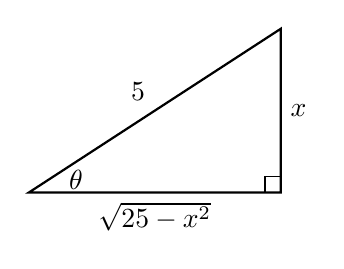
\begin{tikzpicture}[scale=0.8]
        \draw[thick] (0,0) -- (4,0) -- (4,2.6) -- cycle;
        \draw (3.75,0) -- (3.75,0.25) -- (4,0.25);
        \node at (0.75,0.2) {$\theta$};
        \node[above left] at (2,1.3) {$5$};
        \node[right] at (4,1.3) {$x$};
        \node[below] at (2,0) {$\sqrt{25-x^2}$};
      \end{tikzpicture}
      \end{center}
      $\sin\theta = \dfrac{x}{5}$, so $x = 5\sin\theta$ and $dx = 5\cos\theta\,d\theta$.

      $\cos\theta = \dfrac{\sqrt{25-x^2}}{5}$, so $\sqrt{25-x^2} = 5\cos\theta$.
      \[
        \int \frac{5\cos\theta\,d\theta}{25\sin^2\theta\cdot 5\cos\theta}
        = \frac{1}{25}\int \csc^2\theta\,d\theta = -\frac{1}{25}\cot\theta + C.
      \]
      From the triangle, $\cot\theta = \dfrac{\sqrt{25-x^2}}{x}$, so
      \[
        \boxed{\int \frac{dx}{x^2\sqrt{25-x^2}} = -\frac{\sqrt{25-x^2}}{25x} + C}
      \]
    \end{solution}
    \vfill

  \item (8 points) $\ds \int \frac{dx}{x^2-5x+6} $
    \begin{solution}
      $x^2 - 5x + 6 = (x-2)(x-3)$, and
      \[
        \frac{1}{(x-2)(x-3)} = \frac{A}{x-2} + \frac{B}{x-3}
        \quad\Longrightarrow\quad 1 = A(x-3) + B(x-2).
      \]
      $x = 2$: $A = -1$. \quad $x = 3$: $B = 1$.
      \[
        \int\left(\frac{1}{x-3} - \frac{1}{x-2}\right)dx
        = \boxed{\ln|x-3| - \ln|x-2| + C}
      \]
    \end{solution}
    \vfill
  \end{enumerate}

  \newpage

\item BONUS (5 points) Evaluate $\ds \int e^{5x} \sin(7x) \, dx$
  \begin{solution}
    Let $I = \int e^{5x}\sin(7x)\,dx$. Integration by parts with $u = \sin(7x)$,
    $dv = e^{5x}\,dx$,\newline $du = 7\cos(7x)\,dx$, $v = \tfrac15 e^{5x}$:
    \[
      I = \frac15 e^{5x}\sin(7x) - \frac75\int e^{5x}\cos(7x)\,dx.
    \]
    Again with $u = \cos(7x)$, $dv = e^{5x}\,dx$, $du = -7\sin(7x)\,dx$, $v = \tfrac15 e^{5x}$:
    \[
      \int e^{5x}\cos(7x)\,dx = \frac15 e^{5x}\cos(7x) + \frac75 I.
    \]
    Substituting,
    \begin{gather*}
      I = \frac15 e^{5x}\sin(7x) - \frac{7}{25} e^{5x}\cos(7x) - \frac{49}{25} I \\[4pt]
      \text{Solving for } I:\quad
      \frac{74}{25} I = \frac{1}{25}e^{5x}\big(5\sin(7x) - 7\cos(7x)\big).
    \end{gather*}
    \[
      \boxed{\int e^{5x}\sin(7x)\,dx = \frac{e^{5x}\big(5\sin(7x) - 7\cos(7x)\big)}{74} + C}
    \]
  \end{solution}


\end{enumerate}

\end{document}
%%% Local Variables:
%%% mode: LaTeX
%%% TeX-master: t
%%% End:
